\part{Билеты на хор}
\setcounter{section}{0}

\section{Все умения, указанные в вопросах на удовл., но большей сложности (в разумных пределах).}
Всё понятно.

\section{Является ли данное кольцо K коммутативным? областью целостности? полем? Какие в K есть обратимые, неразложимые элементы?}
\begin{itemize}
 \item $K = \Z[i]$

\begin{enumerate}
    \item Это коммутативное кольцо (проверить самостоятельно подстановкой)
    \item Это область целостности (оно ассоциативно + нет делителей нуля, от противного)
    \item Это не поле (например, 2 не обратимо, так как $\frac{1}{2}\notin \Z[i]$)
    \item Обратимые элементы: $\pm 1$, $\pm i$ (те, у которых норма равна 1)
    \item Неразложимые при $|z| < 5$: $ \pm 1 \pm 2i,\; \pm 2 \pm i$
\end{enumerate}

\item $K = \Z[2i]$
\begin{enumerate}
    \item Это коммутативное кольцо (проверить самостоятельно подстановкой)
    \item Это область целостности (оно ассоциативно + нет делителей нуля, от противного)
    \item Это не поле (не у всякого элемента есть обратный)
    \item Обратимые элементы: $\pm 1$ (взять $N(a + 2bi) = a^2 + 4b^2 = 1$)
    \item Неразложимые при $|z| < 5$: $\pm 2,\; \pm 2i,\; \pm 1\pm 2i $
\end{enumerate}

\item $K = \Z[\sqrt{3}i]$
\begin{enumerate}
    \item Это коммутативное кольцо (проверить самостоятельно подстановкой)
    \item Это область целостности (оно ассоциативно + нет делителей нуля, от противного)
    \item Это не поле (не у всякого элемента есть обратный)
    \item Обратимые элементы: $\pm 1$ (взять $N(a + \sqrt{3}bi) = a^2 + 3b^2 = 1$)
    \item Неразложимые при $|z| < 5$: $\pm2, \; \pm\sqrt{3}i,\; \pm1\pm\sqrt{3}i,\; \pm5$
\end{enumerate}

\item $K = \Z[\omega]$
\begin{enumerate}
    \item Это коммутативное кольцо (проверить самостоятельно подстановкой)
    \item Это область целостности (оно ассоциативно + нет делителей нуля, от противного)
    \item Это не поле (не у всякого элемента есть обратный)
    \item Обратимые элементы: $\pm 1, \pm \omega, \pm \omega^2$ 
    (взять $N(a + b\omega) = a^2 -ab + b^2 = 1$)
    \item Неразложимые при $|z| < 5$: $2, 2 + \omega, 3 + \omega, 5 + 2\omega$ с точностью до сопряжения и домножения на обратимый элемент.
\end{enumerate}

\end{itemize}
\newpage{}

\section{Для любого числа $u \in C$ определим множество $Z[u] = \cup\{a_0+a_1u+\ldots+a_nu^n | a_i \in Z\}$.}
Для любого числа $u \in \Comp$ определим множество $\Z[u] = \cup_{n=0}^{\infty}\{a_0+a_1u+\ldots+a_nu^n | \forall i \; a_i \in \Z\}$.
\newline а) Докажите, что $\Z[u]$ является областью целостности. \newline б) При каких $u \in \Comp $ данное $\Z[u]$ «конечномерно
над $\Z$», то есть найдётся такое $N$, что $\Z[u] = \{a_0 + a_1u + \ldots + a_Nu^N | a_0, a_1, \ldots , a_n \in\Z\}$?
\newline \noindent 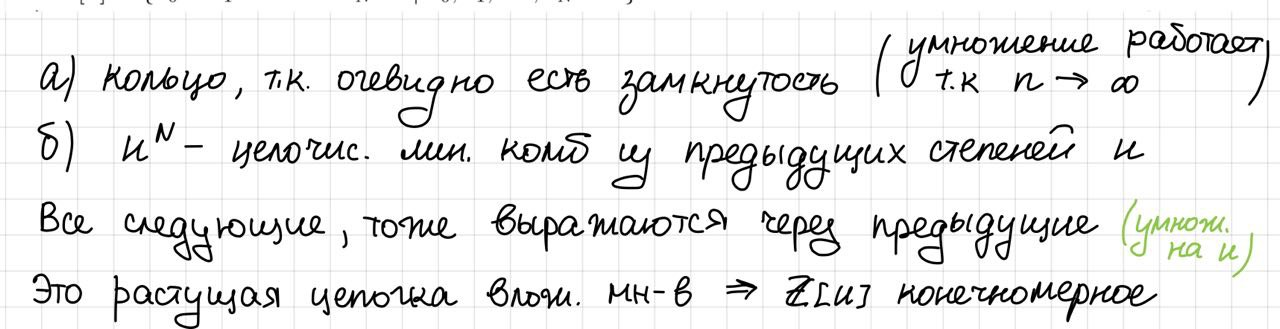
\includegraphics[width=1\linewidth]{sections/Polya/х3.jpg}
\newline \noindent 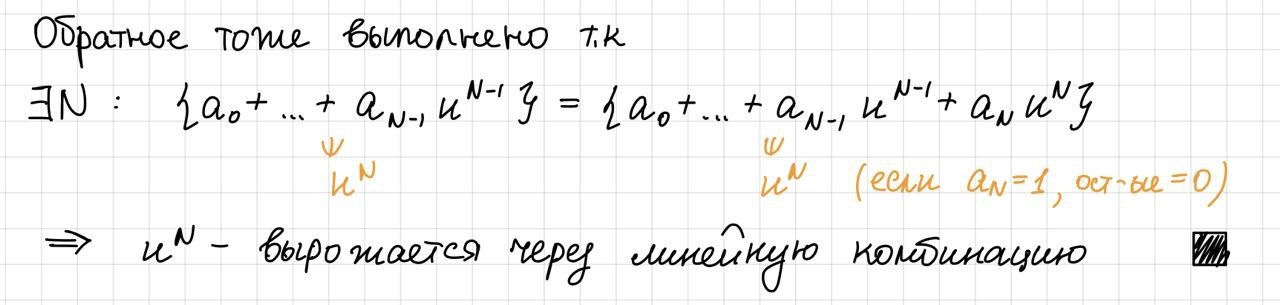
\includegraphics[width=1\linewidth]{sections/Polya/х3_2.jpg}

\section{В конечном коммутативном кольце если элемент не является делителем нуля, то он обратим.}
\noindent 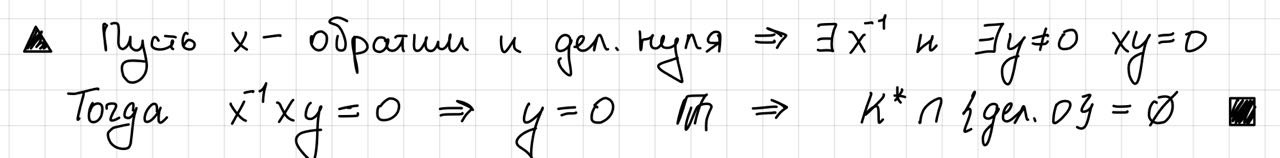
\includegraphics[width=1\linewidth]{sections/Polya/х4.jpg}

\section{Конечная область целостности (состоящая из более чем одного элемента) — поле.}
\noindent 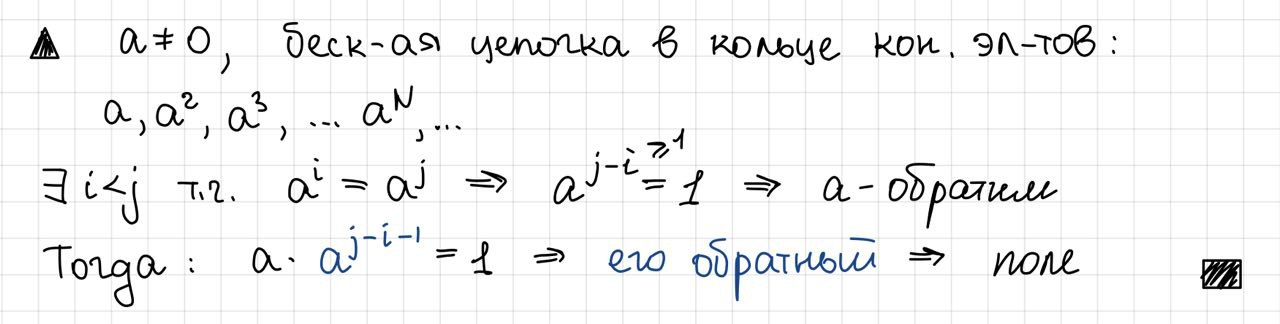
\includegraphics[width=1\linewidth]{sections/Polya/х5.jpg}

\section{Числа Эйзенштейна}
$|a + b \omega| = \sqrt{a^2 - ab + b^2}$
(красным выделены обратимые, $Z^*[w]$

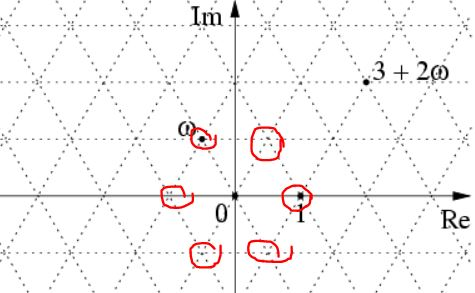
\includegraphics[]{images/4_6.JPG}


\section{Пример нефакториального кольца вида Z[u].}
Область целостности $K$ называется \textit{факториальным кольцом}, если для всех $x \in K \backslash \{0\}$ выполнены условия:
	\begin{enumerate}
		\item $x$ представим в виде $x = up_1\dotsm p_s$, где $u \in K^*$, $p_1, \dotsc, p_s$ "--- неразложимые (разложение $x$ \textit{существует})
		\item если $x = up_1\dotsm p_s = wq_1 \dotsm q_l$, где $u, w \in K^*$, $p_1, \dotsc, p_s, q_1, \dotsc, q_l$ "--- неразложимые, то $l = s$ и $\exists \sigma \in S_s: \forall i \in \{1, \dotsc, s\}: p_i \sim q_{\sigma(i)}$ (разложение $x$ \textit{единственно})
	\end{enumerate}
	
Покажем, что $\Z[2i]$ не является факториальным кольцом. Аналогично случаю $\Z[i]$ можно показать, что $\Z[2i]^* = \{\pm1\}$, и элементы $2, 2i$ неразложимы. Тогда $4 = 1 \cdot 2 \cdot 2 \hm= (-1)\cdot (2i) \cdot (2i)$, но $2 \not\sim 2i$.


\section{Условие $N(ab) > N(b)$ из определения евклидова кольца не существенно}
\Proof 
	Пусть $K$ "--- область целостности, $N: K \backslash \{0\} \to \N \cup \{0\}$ "--- функция со свойством деления с остатком. Для $\forall a \in K \backslash \{0\}$ положим $\overline{N}(a) := \min\{N(ab) : b \in K \backslash \{0\}\}$. Проверим, что для $\overline{N}$ выполнены оба свойства нормы:
	\begin{enumerate}
		\item Заметим, что $\forall a, b \in K \backslash \{0\}: \overline{N}(ab) = N(abc)$ для некоторого $c \in K \backslash \{0\}$. Тогда $\overline{N}(ab) \ge \min\{N(ax) : x \in K \backslash \{0\}\} = \overline{N}(a)$.
		\item Пусть $a, b \in K \backslash \{0\}$. Выберем такой $x \in K \backslash \{0\}$, что $\overline{N}(b) = N(bx)$, и поделим $a$ на $bx$ с остатком: $a = bxq + r$, где либо $r = 0$, либо $N(r) < N(bx)$. Остается заметить, что тогда $\overline{N}(r) \le N(r) < N(bx) = \overline{N}(b)$.\qedhere
	\end{enumerate}
\EndProof
\newpage{}

\section{Геометрическое доказательство евклидовости.}

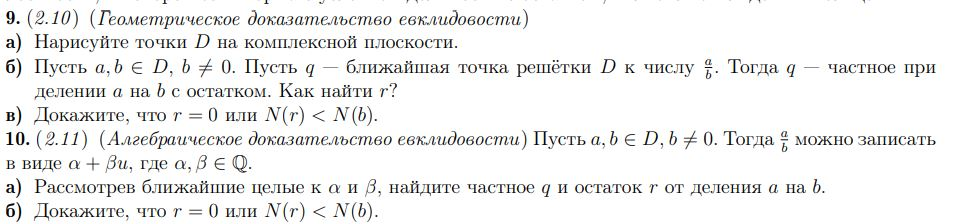
\includegraphics[scale=0.9]{images/4_9_10.JPG}

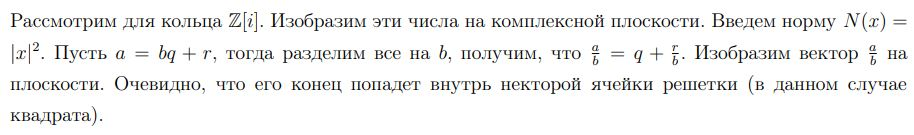
\includegraphics[scale=0.95]{images/4_9_1.JPG}

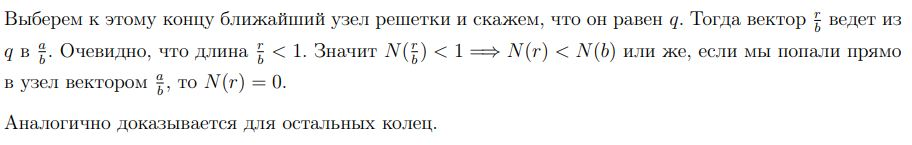
\includegraphics[scale=0.95]{images/4_9_2.JPG}

\section{Алгебраическое доказательство евклидовости.}

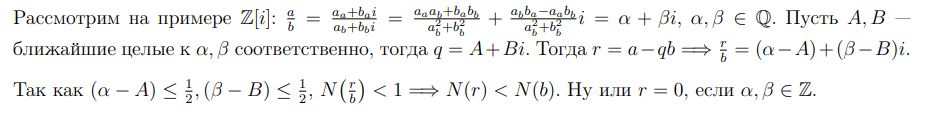
\includegraphics[scale=0.95]{images/4_10.JPG}
\newpage{}

\section{Алгоритм Евклида в евклидовом кольце.}
Пусть $K$ — евклидово кольцо. Тогда а) Алгоритм Евклида в $K$ остановится. б) Последний не нулевой элемент $r_n$ в алгоритме Евклида — делитель $a$ и $b$. в) Найдутся такие $x, y \in K$, что $r_n = ax + by$. г) Определим наибольший общий делитель $a$ и $b$ как делитель $a$ и $b$ максимальной нормы. Тогда $r_n$ — наибольший общий делитель

\Proof

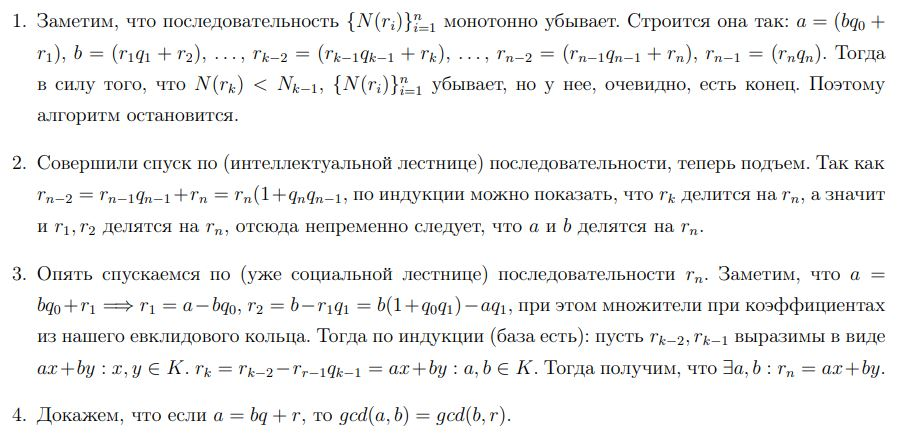
\includegraphics[scale=0.95]{images/4_11_1.JPG}

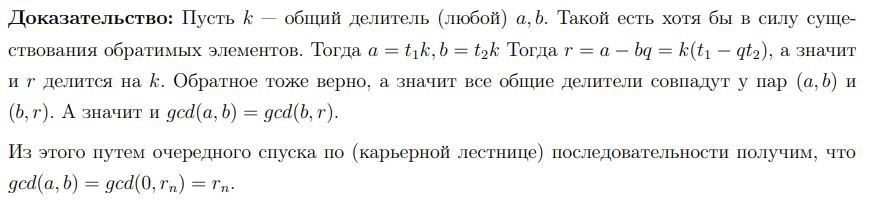
\includegraphics[scale=0.95]{images/4_11_2.JPG}

\EndProof
\newpage{}

\section{В факториальном кольце любой неразложимый элемент является простым.}
\Def $p \in K$ — простой, если из того, что $ab$ делится на $p$, следует, что либо  $a$ делится на $p$, либо $b$ делится на $p$.

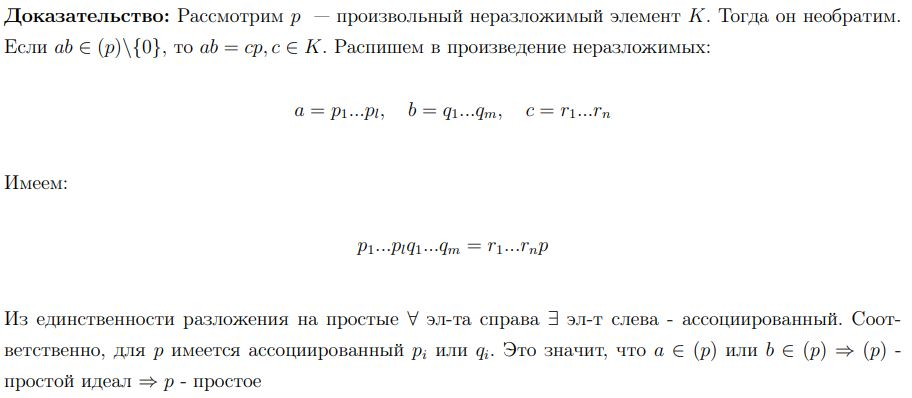
\includegraphics[scale=0.95]{images/4_12.JPG}

\section{Если в области целостности K существует разложение в произведение неразложимых элементов и любой неразложимый элемент прост, то K факториально}
\Proof Достаточно доказать единственность разложения. \newline Пусть $x \in K\backslash \{0\}$ и $x = up_1 ... p_s = wq_1...q_l$, где $u$, $w$ $\in K^*$, $p_1,... , p_s, q_1, ... , q_l$ -- неразложимые.
\newline Пусть $s$ -- наименьшее, то есть в разложении $x$ участвует наименьшее количество неразложимых элементов, среди всех элементов с неединственным разложением. \newline Поскольку элемент $p_1$ -- простой, то или $p_1 | w$, или $p_1 | q_1$, ... , или $p_1 | q_l$. Первое невозможно, поскольку $p_1 \not\in K^*$, поэтому $p_1 | q_i$ для некоторого $i \in \{1, ..., l\}$. Поскольку $q_i$ -- неразложимый, то $p_1 \sim q_i$, поэтому обе части равенства можно сократить на $p_1$. Но тогда разложение элемента $up_2 ... p_s$
неединственно, что противоречит минимальности $s$. \EndProof

\section{Евклидово кольцо факториально.}
Пусть K - евклидово кольцо \\ \\
\Lemma  У каждого элемента $x \in K\backslash \{0\}$ существует разложение
\\
\Proof Предположим, что это не так и рассмотрим элемент $x \in K\backslash \{0\}$ с минимальной нормой, который не раскладывается в произведение неразложимых. Представим $x$ в виде $x = ab$, где $a$, $b$ $\in K\backslash \{0\}$, тогда $N(x) > N(a)$, $N(x) > N(b)$.
\\
Если оба неравенства строгие, то разложение элемента $x$ существует как произведение разложений элементов $a, b$ -- противоречие. 
\\
Пусть теперь $N(ab) = N(a)$. Разделим $a$ на $ab$ с остатком: $a = q(ab)+r, \;q, r \in K$. 
\begin{itemize}
    \item Если $r = 0$, то $bq = 1$ и $b$ обратим.
    \item  Если же $N(r) < N(ab)$,
то $N(ab) > N(r) = N(a(1 - q b)) > N(a)$,
что невозможно.
\end{itemize}
 Случай, когда $N(ab) = N(b)$, аналогичен.
\\
Таким образом, для всех представлений $x$ в виде $x = ab$, $a$, $b$ $\in K\backslash \{0\}$, один из элементов
$a$, $b$ -- обратимый, поэтому $x$ -- неразложимый элемент, и у него есть разложение $x = 1 \cdot x$.\\
Снова получено противоречие. \EndProof
\bigbreak 
\noindent \Lemma (Евклида) Каждый неразложимый элемент $p$ в $K$ прост, то есть $\forall a, b \in K : p | ab \Longrightarrow p | a $ лии $p | b$.
\\
\Proof Если $p | a$, то утверждение уже доказано. Предположим, что $p \nmid a$,
и докажем, что $\exists x, y \in K : a x + p y = 1$. Для этого рассмотрим следующий процесс последовательного деления с остатком, называемый алгоритмом Евклида:
\begin{itemize}
    \item []$a = p q_1 + r_1$
    \item [] $p = r_1q_2 + r_2$
    \item [] $r1 = r_2 q_3 + r_3$
    \item[] ...
\end{itemize}
Поскольку N($p$) > N($r_1$) > N($r_2$) > . . . , то $\exists k \in \N : r_{k+1} = 0$. Значит, $r_{k-1} = r_k q_{k+1}$, и легко по индукции убедиться, что тогда $r_k | a$ и $r_k | p$. Поскольку p неразложим и $p \nmid a$, то
$r_k \sim 1$. По индукции получим, что $\exists \ x, y \in K : a x + p y = 1$, тогда $abx + pby = b$ и $p | b$.\EndProof
\\
\\
\Th  Кольцо K факториально \\
\Proof В K существует разложение для каждого ненулевого элемента, и каждый неразложимый элемент в K прост по лемме Евклида, поэтому K факториально. \EndProof

\section{Если D — факториальное кольцо, то для любого неразложимого элемента z $\in$ D либо N(z) = p, либо z $\sim$ p для некоторого целого простого числа p}
\ \\$D$ = Z[$u$], где $u \in \{i, \omega, \sqrt{2}i\}.$ Норма в Z[$u$] мультипликативна, то есть $\forall a, b \in$ Z[$u$] : N($ab$) = N($a$)N($b$).
\\ 
\\
\Proof Пусть x неразложим. Тогда $x$ прост, и, поскольку $N(x) = x\overline{x}$, $x | p$, где $p$ — некоторый простой делитель N($x$), то есть $p$ = $xw$ для некоторого $w \in D$, и N($x$)N($w$) = N($p$) = $p^2$. Если N($x$) = 1, то $x$ обратим, что невозможно. Если N($x$) = $p$, то
получено требуемое. Если же N($x$) = $p^2$, то N($w$) = 1, то есть w обратим, поэтому
$x \sim p$ и $p$ неразложим. \EndProof
\newpage 
\section{Следующие простые натуральные числа являются неразложимыми}
а) числа вида
$p = 4k + 3$ в $\Z[i]$; 

б) числа вида $p = 3k + 2$ в $\Z[\omega]$. 
в) числа вида $p \equiv −1,−3 (mod 8)$ в $\Z[\sqrt{2}i]$.

\noindent 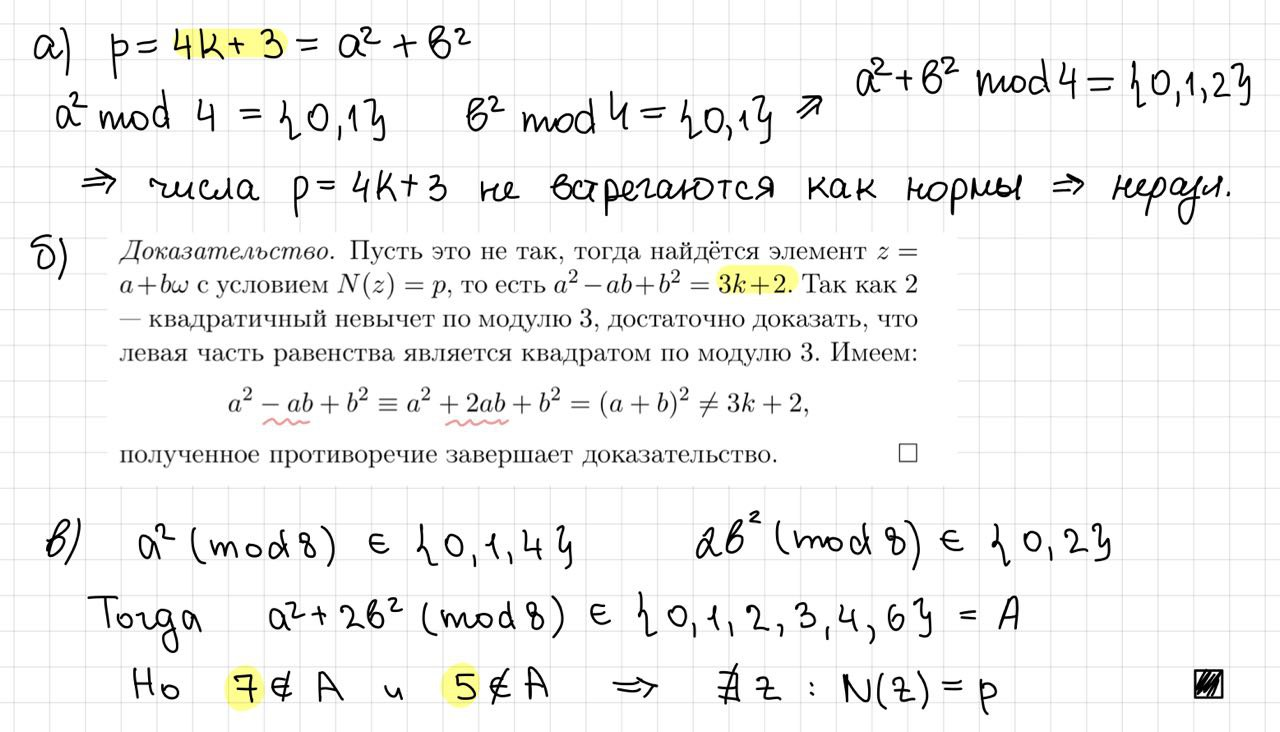
\includegraphics[width=1\linewidth]{sections/Polya/х16.jpg}

\section{Описание представления натурального числа в виде суммы двух квадратов (доказательство,
использующее гауссовы целые числа).}
\ \\\textbf{Утверждение} Натуральное число представимо в виде суммы двух квадратов тогда и только тогда, когда любое простое число вида 4k + 3 входит в его разложение на простые множители в четной степени.
\\
\Proof 
\\
$\Rightarrow$ Пусть $n$ = $a^2$ + $b^2$. Тогда n =  $(a + i b)(a - i b) = z\overline{z}$. Разложим $z$ на простые гауссовы числа: $z = up_1...p_s * q_1...q_l$, где $p_1...p_s$ -- простые целые числа вида 4k+3, а $q_1...q_l$ -- простые гауссовы числа, имеющие ненулевую мнимую часть. Такое разложение возможно, так как все простые числа имеют вид либо 4k+3, либо 4k+1, и последнее представимо в виде произведения гауссовых чисел и u, $u \in \{\pm 1, \pm i\}$. Тогда имеем:
\begin{center}
    $\overline{z} = \overline{up_1....p_sq_1....q_l} = p_1...p_s\overline{u}\ \overline{q_1}....\overline{q_l}$ 
\end{center}
Следовательно $n = z\overline{z} = p_1^2...p_s^2u \overline{u} q_1\overline{q_1}...q_l\overline{q_l} = p_1^2...p_s^2N(q_1)...N(q_l)$ - разложение на простые множители. \\
$\Leftarrow$ $n = p_1^2...p_s^2N(q_1)...N(q_l)$. Пусть $z = p_1..p_s q_1...q_l \longrightarrow \overline{z} = p_1...p_s \overline{q_1}...\overline{q_l}$ и $n = z\overline{z} = a^2 + b^2$, если $z = a+ i b$ \EndProof


\section{Пусть $D = Z[i]$ или $Z[\omega]$. Утверждения про норму:} 
\noindent а) Верно ли, что из $a | b$ следует, что $N(a) | N(b)$? б) Верно ли, что
из $(N(a),N(b)) = 1$, следует $(a, b) = 1$? 
\\
в) Пусть $(N(a),N(b)) = p$ -- простое целое число, причём $p$ не делит $a$,
$p$ не делит $b$. Тогда $p$ -- разложим, и если $p = z\overline{z}$, то либо $z$, либо $\overline{z}$ порождает идеал $(a, b)$, либо $z$ делит одно из
этих чисел, а $\overline{z}$ — другое.
\newline \noindent 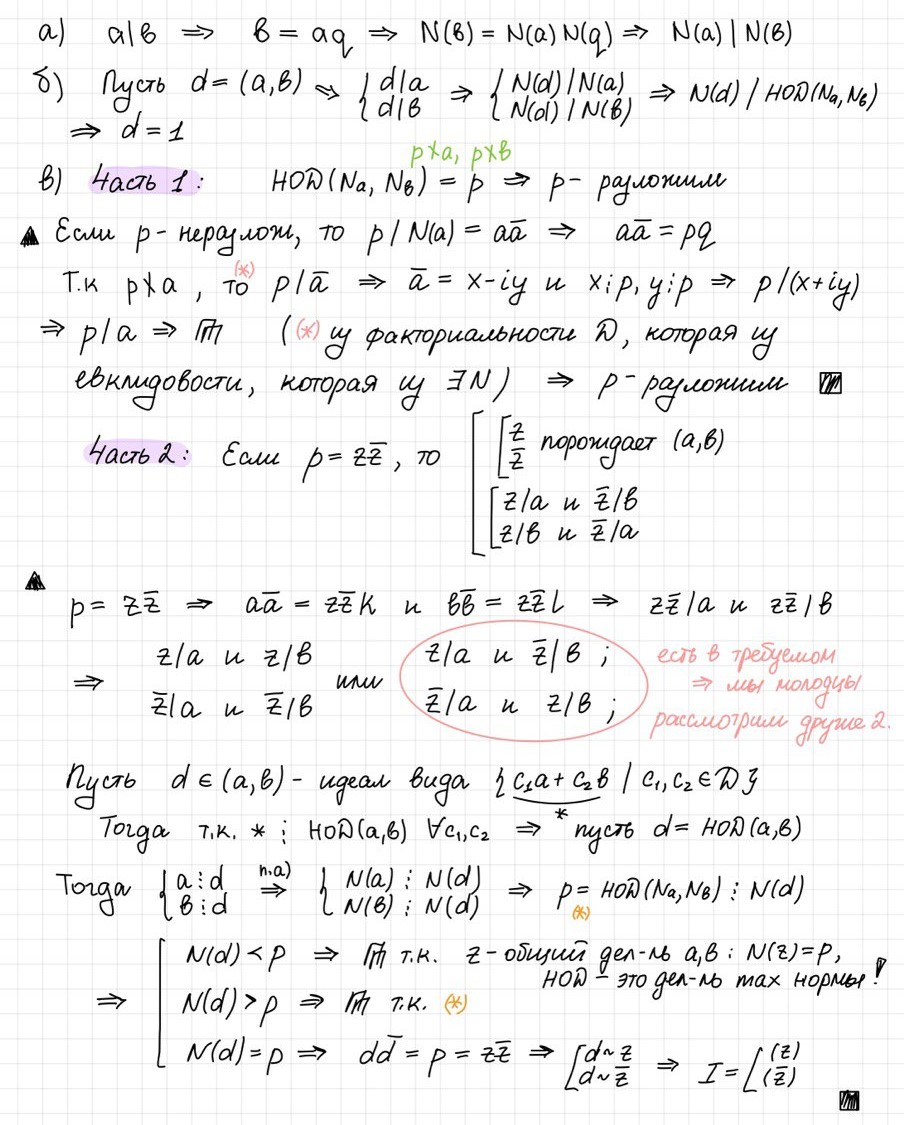
\includegraphics[width=0.95\linewidth]{sections/Polya/х18.jpg}

\section{Пусть $K$ -- коммутативное кольцо. Являются ли идеалом:
а) множество нильпотентных элементов $N(K) = \{a \in K | \exists m \in N : a^m = 0\}$;
б) радикал $\sqrt{I} = \{a \in K | \exists m \in N : a^m \in I\}$ идеала I?}
 \noindent 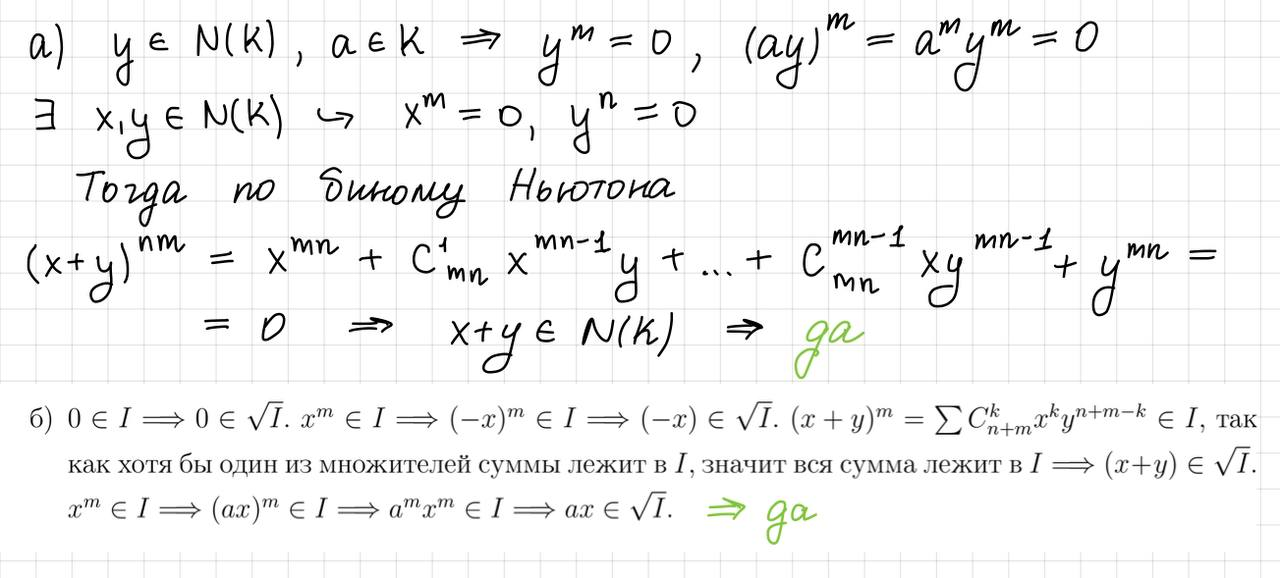
\includegraphics[width=1\linewidth]{sections/Polya/х19.jpg}

\section{а) Идеал $(x, y)$ кольца $Q[x, y]$ конечно порождён, но не является главным. б) Приведите
пример области целостности $K$ и идеала $I$, который не конечно порождён.}
\noindent 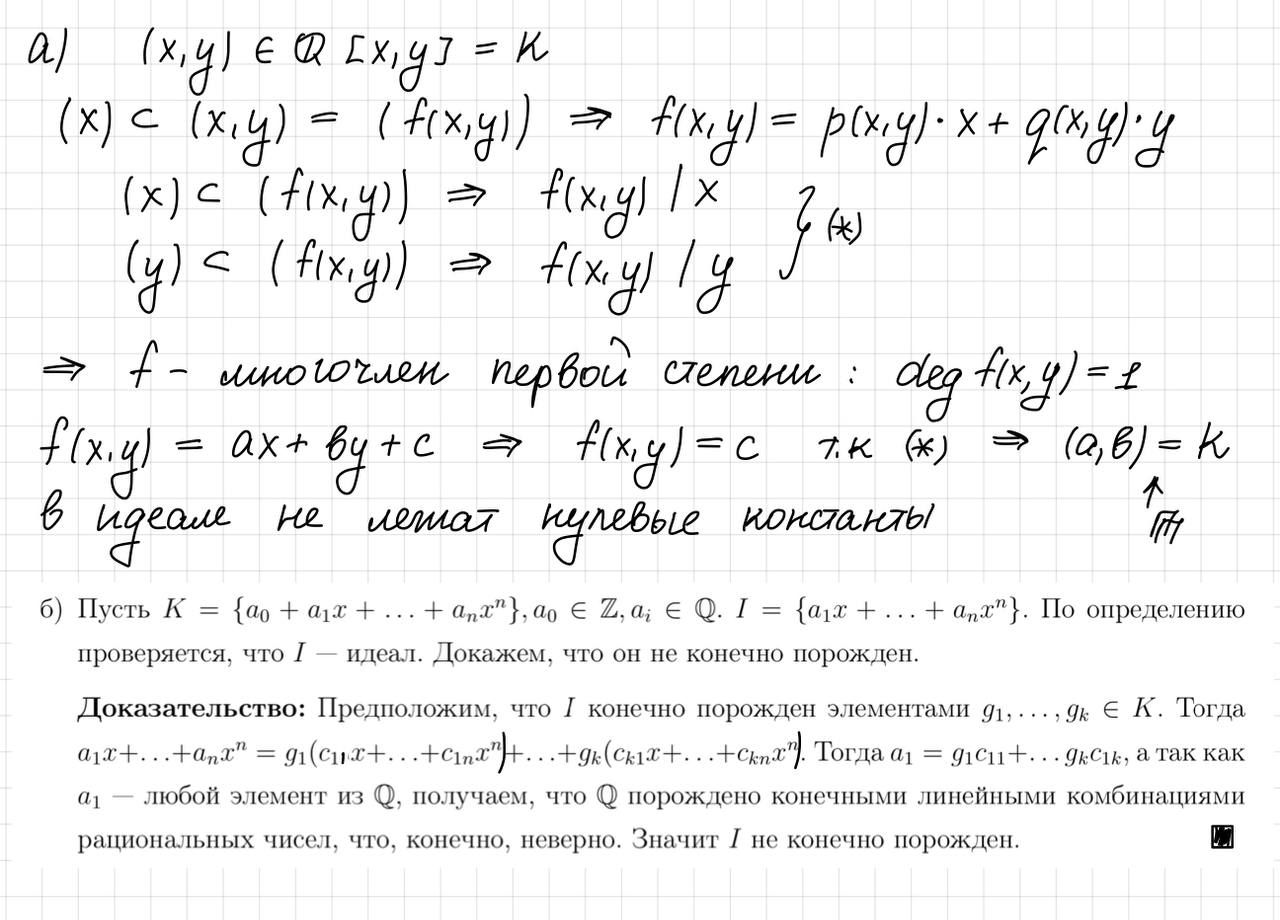
\includegraphics[width=1\linewidth]{sections/Polya/х20.jpg}

\section{Евклидово кольцо является кольцом главных идеалов.}
\noindent 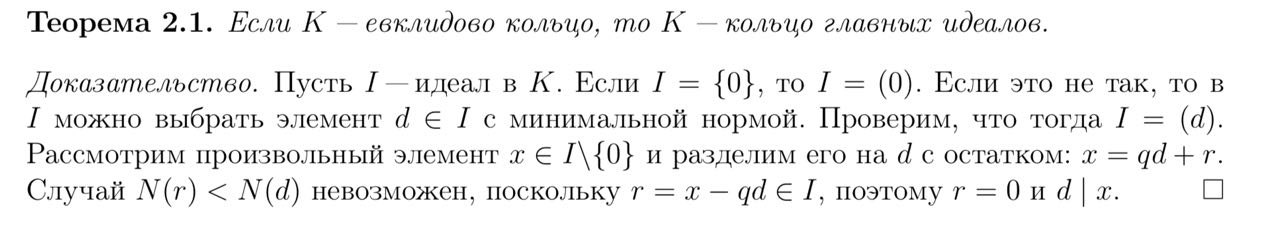
\includegraphics[width=1\linewidth]{sections/Polya/х21.jpg}

\section{ Пусть K — кольцо главных идеалов.
а)  Любая цепочка возрастающих идеалов стабилизируется, то есть из того, что $I_1 \subset I_2 \subset I_3 \subset . . . \subset I_n \subset . . .$
(где все $I_k$ — идеалы) следует, что найдётся такое n, что $I_n= I_{n+1} = ...$
б) В $K$ существует разложение в произведение неразложимых (в смысле 1-й части определения факториального кольца).}
\ \\ 
Пусть K — кольцо главных идеалов.

\textbf{Утверждение:} Любая цепочка возрастающих идеалов стабилизируется, то есть из того, что $I_1 \subset I_2 \subset I_3 \subset . . . \subset I_n \subset . . .$
(где все $I_k$ — идеалы) следует, что найдётся такое $n$, что $I_n= I_{n+1} = ...$
\\
\Proof
Пусть $(a_0) \subset (a_1) \subset(a_2) \subset...$— возрастающая последовательность идеалов в K. Проверим, что $I := \bigcup\limits_{i=0}^{\infty}(a_i)$ — тоже идеал. Действительно, если b, c $\in$ $I$, то
$b$, $c \in (a_k)$ для некоторого $k \in \N$, \newline поэтому $b$ + $c \in (a_k) \subset I$ и $\forall x \in K : bx, c x \in (a_k) \subset I$.
\newline Поскольку $K$ — кольцо главных идеалов, то $I = (y)$ для некоторого $y\in K$. Но тогда
$y  \in (a_m)$ для некоторого $m \in \N$, поэтому последовательность стабилизируется, начиная с номера $m$, то есть $\forall n \geq m : I_n = I_m$.\EndProof
\bigbreak
\textbf{Утверждение: } В $K$ существует разложение в произведение неразложимых (в смысле 1-й части определения факториального кольца).
\\
\Proof Предположим, что это неверно для элемента $a \in K \backslash \{0\}$. Тогда $a$ можно
представить в виде $a = a_1 b_1$, где $a$, $b_1 \not\in K^* \cup \{0\}$, и у $a_1$ тоже нет разложения. Повторяя этот процесс для $a_1$, $a_2$, . . . , получим последовательность идеалов ($a$) $\subset$ ($a_1$) $\subset$ ($a_2$) $\subset$ ... ,
причем все вложения в ней строгие к силу попарной неассоциированности порождающих
элементов. Это противоречит тому, что последовательность должна стабилизироваться.
Значит, разложение есть у каждого ненулевого элемента.\EndProof


\section{В кольце главных идеалов любой неразложимый элемент является простым}
Пусть $K$ -- кольцо главных идеалов, $p$ — неразложимый элемент $K$, 
$ab$ делится на $p$, $a$ не делится на $p$. 
Рассмотрим $I$ -- множество таких элементов $x \in K$, 
что $ax$ делится на $p$.

\underline{а) $I$ -- идеал.}

Если $x, y \in I$, то $x + y \in I$, так как 
$ax\ \vdots\ p, ay\ \vdots\ p \Rightarrow a (x + y)\ \vdots\ p$.

$\forall k \in K \ \ \forall x \in I \ \ kx \in I$, так как
$ax\ \vdots\ p \Rightarrow a(kx)\ \vdots\ p$.

\underline{б) $1 \not \in I, p \in I, b \in I$}

$1 \not \in I$, так как $a \cdot 1 = a\ \cancel{\ \vdots\ }\ p$.

$p \in I$, так как $a \cdot p\ \vdots\ p$.

$b \in I$, так как $ab\ \vdots\ p$.

\underline{в) $I = (p)$}

Так как $K$ -- кольцо главных идеалов, то $\exists y \in K\ :\ I = (y)$.
\newline $p \in I$, следовательно, $\exists k \in K\ :\ p = ky$.
Так как $p$ -- неразложимый, то либо

1) $k$ обратим -- Тогда $p \sim y$, то есть $I = (p)$.

2) $y$ обратим -- Но тогда идеал, порождённый $y$, совпадает со всем кольцом, а значит
содержит и единицу (противоречие с пунктом б).

\underline{г) $b$ делится на $p$}

$I$ содержит элементы, которые делятся на $p$, а $b \in I$.
Следовательно, $b$ делится на $p$.

\underline{д) Любой неразложимый элемент $K$ является простым.}

Пусть $p \in K$ неразложим, 
тогда для любых $a, b \in K\ :\ ab\ \vdots\ p$ верно что либо 
$a\ \vdots\ p$, либо $b\ \vdots\ p$ (по пункту г)).



\section{ Доказательство эквивалентности определений (3 штуки) нётеровых колец}
 \Def Область целостности $K$ называется \textit{нетёровым кольцом}, если выполнено одно из следующих условий:
\begin{itemize}
    \item [1] Если $I_0 \subset I_1 \subset I_2 \subset . . . $ -- последовательность идеалов в $K$, то $\exists \ m \in \N : \forall \ n \geqslant m :I_n = I_m$.
    \item [2] Любой идеал в $K$ является конечнопорожденным.
    \item[3] Если $(a_0) \subset (a_0, a_1) \subset (a_0, a_1, a_2) ... $ - последовательность идеалов в $K$, то $\exists m \in \mathbb{N} \ \forall \ n \geq m: \ a_n \in (a_1, ..., a_m)$
\end{itemize}
\Proof
 \begin{itemize}
     \item []$(1 \Longrightarrow 3)$  Тривиально, это частный случай более общего утверждения.
       \item []$(3 \Longrightarrow 2)$ Пусть $I$ - ненулевой идеал в $K$. Выберем $a_0 \in I$. \newline Если $I = (a_0)$, то получено требуемое. \newline Иначе -- выберем $a_1 \in I\backslash (a_0)$. Если $I = (a_0, a_1)$, то получено требуемое. Иначе -- выберем $a_2 \in I\backslash (a_0, a_1)$ и продолжим процесс. Предположим, что этот процесс не завершается, тогда в $I$ есть нестабилизирующаяся последовательность идеалов $(a_0) \subset (a_0, a_1) \subset (a_0, a_1, a_2) \subset ...$ , что невозможно.
       \item []$(2 \Longrightarrow 1)$ Пусть $I_0 \subset I_1 \subset I_2 \subset . . .$ -- последовательность идеалов в $K$. Как уже было
доказано, $I :=  \bigcup\limits_{j=0}^{\infty} I_j$ - тоже идеал (билет 4.22), тогда $I$ конечнопорожден, то есть $I = (a_1, . . . , a_n)$
для некоторых $a_1, . . . , a_n \in K$. Но тогда $\exists m := $min$\{j \in \Z_{\geqslant 0} : a_1, . . . , a_n \in I_j\} :
\forall n \geq m : I_n = I_m.$
 \end{itemize}
 \EndProof

\section{В нётеровом кольце существует разложение в произведение неразложимых элементов (условие (1)
факториального кольца).}
Идейно: доказательство аналогично доказательству для кольца главных идеалов, т.к. в нетеровых кольцах цепочки вложенных друг в друга идеалов также стабилизируются.

\Proof
Пусть $K$ -- наше кольцо.
Пусть $a$ -- ненулевой элемент, для которого нет разложения на неразложимые элементы, при этом сам $a$ является разложимым ( иначе есть разложение $a = a$). Тогда $a = a_1b : a_1, b \not\in K^*\cup\{0\}$, при этом $a_1$ не представляется в виде неразложимых. Тогда $(a) \varsubsetneq (a_1)$ Аналогично получаем
цепочку $(a) \varsubsetneq (a_1) \varsubsetneq (a_2) \varsubsetneq \ldots$

(Включения строгие в силу попарной неассоциированности порождающих элементов)

Получаем цепочку, которая не стабилизируется, противоречие с нетеровостью.

\EndProof

\section{(7.4) а) Верно ли, что $Quot(Quot(K))$ изоморфно
$Quot(K)$? б) Пусть $K \subset L \subset Quot(K)$. Верно ли, что
$Quot(K)$ изоморфно $Quot(L)$?}
\textbf{а)} Рассмотрим $\frac{a}{b} \in Quot(Quot(K))$, где $a, b \in Quot(K)$. Т.к. $Quot(K)$ -- поле, то $\frac{a}{b} \in Quot(K)$. Тогда можно поставить в соответствие элемент $\frac{(\frac{a}{b})}{e}$ (где $e$ -- единичные элемент) из $Quot(Quot(K))$ и $\frac{a}{b}$ из $Quot(K)$. Получим изоморфизм.

\textbf{б)}

Воспользуемся универсальным свойством. Но для этого сначала его напомниим:

Пусть у нас есть вложение $f: K \to L$, $L$ -- поле. Также у нас есть вложение $i: K \to Quot(K)$. В этом случае существует единственное вложение $\phi: Quot(K) \to L$, которое продолжает $f$, то есть $\phi \circ i = f$.

Легко понять, как строится это вложение:

Воспользуемся тем, что $L$ поле. Тогда если $f(a) \in L \Rightarrow f(a)^{-1} \in L$, поэтому положим $\phi(\frac{a}{b}) = f(a)f(b)^{-1}$\\

Теперь вернемся к нашей задаче. Можно построить следующие вложения: $i_1: K \to L, i_2: L \to Quot(K), \alpha: K \to Quot(K), \beta: L \to Quot(L)$. Теперь несколько раз воспользуемся универсальным свойством, а именно можно построить инъекцию $\psi: Quot(K) \to Quot(L)$ (в качестве отображения $f$ берем $\beta \circ i_1$), а также $\phi: Quot(L) \to Quot(K)$. В итоге получим две инъекции: $\phi, \psi$ между $Quot(K)$ и $Quot(L)$. Значит, они изоморфны.



\section{(7.8)
а) Пусть $f$ -- примитивный многочлен из $Z[x]$. Если $f(x)$ неприводим в $Z[x]$, то он неприводим и в $Q[x]$.
б) Примитивный неприводимый многочлен $f \in Z[x]$ является простым элементом этого кольца.}
\textbf{а)}
\Proof
Пусть $f$ приводим над $\mathbb{Q}[x]$, то есть $f = gh$, причем $g, h \in \mathbb{Q}[x]$. Тогда $g = \frac{a}{b}g_1, h = \frac{c}{d}h_1$, где $g_1, h_1$ примитивные многочлены степени $\geq 1$ (и из $Z[x]$). Из билета 35 произведение примитивнх многочленов -- примитивный многочлен.

Тогда $f = \frac{ac}{bd}(g_1h_1)$, и (т.к $f, g_1h_1$ примитивны), то $\frac{ac}{bd} = 1$. Тогда $f$ приводим над $\mathbb{Z}[x]$, противоречие.
\EndProof

\textbf{б)}
\Proof
$f(x)$ примитивен, неприводим в $\mathbb{Z}[x]$, значит, неприводим в $\mathbb{Q}[x]$. В $\mathbb{Q}[x]$ это эквивалентно простоте. 

Пусть $f(x)|(g(x)h(x)), g, h \in \mathbb{Z}[x]$. Тогда в $\mathbb{Q}[x]$ один из них делится на $f$, пусть это $g(x)$ (без ограничения общности). Тогда $g(x) = f(x)a(x)$. Заметим, что $g(x) = bg_1(x), g_1(x)$ -- примитивный (в $\mathbb{Z}[x]$). А еще $a(x) = \frac{c}{d}a_1(x), a_1(x)$ -- примитивный (в $\mathbb{Z}[x]$).

Значит, $bdg_1(x) = ca_1(x)f(x)$. Произведение $a_1$ и $f$ -- примитивный многочлен. Тогда $bd = c$, и $g_1(x) = a_1(x)f(x)$. Значит, $f|g_1$, и $f|g$ в $\mathbb{Z}[x]$
\EndProof

\section{Признак неприводимости Эйзенштейна (формулировка + доказательство).}
\noindent 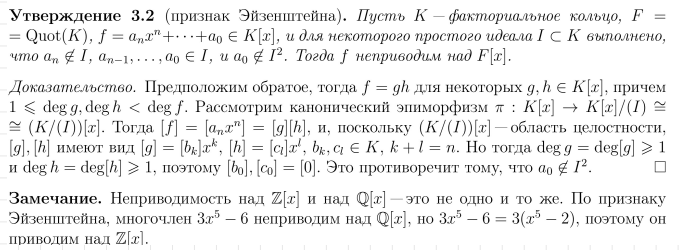
\includegraphics[width=1\linewidth]{sections/Polya/x28.png}

\section{Верно ли, что если $f(x)$ неприводим над $Z_p$ для некоторого простого p, то он неприводим
над $Q$?}
% Рассмотрим многочлен $(2x + 1)(x^2 + x + 1)$. 
% \\ В $\Z_2$ он неприводим, так как многочлен $(x^2 + x + 1)$ не имеет корней в $\Z_2$. Но при этом он приводим над $\Q$ 

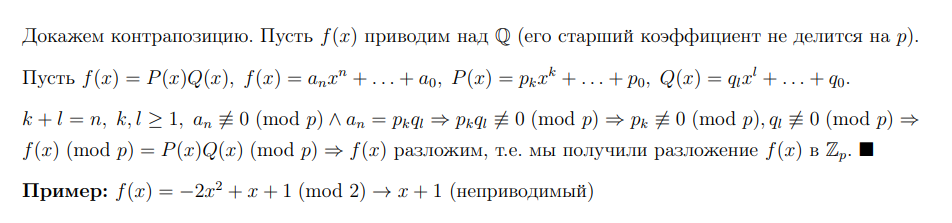
\includegraphics[scale=0.8]{images/4.29.png}

\section{Умение применять критерий Эйзенштейна (в том числе, используя замену переменной)}
См билет 37 на хор (там замена переменных тоже есть)

\section{(9.2) а) $F(\alpha_1, \ldots , \alpha_n)$ корректно определено. б) Верно ли, что $F(\alpha_1, \ldots , \alpha_n)$ изоморфно $Quot F[\alpha_1, \ldots , \alpha_n]$?}
\textbf{а)}
Пусть $F \subset L, \alpha_1, \ldots, \alpha_n \in L$. Тогда $F(\alpha_1, \ldots, \alpha_n)$ -- минимальное по включению поле, содержащее $\alpha_1, \ldots, \alpha_n, F$. Зададим $F(\alpha_1, \ldots, \alpha_n) = \cap K : F \subset K \subset L, \alpha_1, \ldots, \alpha_n \in K$.

\textbf{б)}

Рассмотрим $F' = \{\frac{f(\alpha_1, \ldots, \alpha_n)}{g(\alpha_1, \ldots, \alpha_n)}| f, g \in F[x_1, \ldots, x_n]\}$. С одной стороны, это множество -- поле. С другой, любое поле, содержащее $F, \alpha_1, \ldots, \alpha_n$, обязано его содержать. Из этого следует, что $F(\alpha_1, \ldots, \alpha_n) \cong F' \cong Quot(F[\alpha_1, \ldots, \alpha_n])$
\newpage

\section{Эквивалентность двух определений алгебраического элемента}
$F \subset K$ -- расширение полей,  $\alpha \in K$

Следующие условия эквивалентны:

\begin{enumerate}
    \item $[F(\alpha):F]$ -- конечное
    \item $\exists f(x) \in F[x]$, т.ч. $f(\alpha) = 0$
\end{enumerate}

\Proof

\begin{itemize}
    \item В одну сторону довольно очевидно:
    
    Если  $[F(\alpha):F] = N < \infty$, то $1, \alpha, \ldots, \alpha^N$ ЛЗ над $F$. \newline Тогда $a_0 + a_1\alpha + \ldots a_N\alpha^N = 0, a_0, \ldots, a_N \in F$. \newline Тогда можно взять многочлен $f(x) = a_0 + a_1x + \ldots a_Nx^N$, который будет обнуляться для $x=\alpha$. Значит, $\alpha$ -- алгебраический.
    
    \item $M = \{g(x) \in F[x]\;|\; g(\alpha) = 0\}$. $M$ непусто, т.к. $\alpha$ -- алгебраический.\\
    
    Докажем, что $M$ -- простой идеал в $F[x]$:
    
    \begin{enumerate}
        \item $g, h \in M \Rightarrow (g + h)(\alpha) = g(\alpha) + h(\alpha) = 0 + 0 = 0$
        \item $g \in M, h \in F[x] \Rightarrow (gh)(\alpha) = g(\alpha)h(\alpha) = 0$ (т.к. $g(\alpha) = 0$)
        \item $(gh) \in M \Rightarrow g(\alpha)h(\alpha) = (gh)(\alpha) = 0 \Rightarrow g(\alpha) = 0$ или $h(\alpha) = 0$, т.е. один из них $\in M$
    \end{enumerate}
    
    Тогда $F(\alpha) \cong F[\alpha] \cong F[x]/(m_{\alpha}(x))$
\end{itemize}

\EndProof

\section{(9.8) а) Для данного элемента $\alpha \in K$ и многочлена $f$ со старшим коэффициентом $1$ следующие
условия эквивалентны:...}
\textbf{(9.8 ) а) Для данного элемента $\alpha \in K$ и многочлена $f$ со старшим коэффициентом $1$ следующие
условия эквивалентны:
(1) $f$ порождает идеал $M_{\alpha} = M_{\alpha,F} = \{f(x) \in F[x] | f(\alpha) = 0\}$;
(2) $f$ -- многочлен из $M_{\alpha}$ минимальной степени;
(3) $f$ -- неприводимый многочлен из $M_{\alpha}$.
б) $m_{\alpha}$ -- единственный многочлен, обладающий данными свойствами;
в)  $F(\alpha) \cong F[\alpha] \cong F[x]/(m_{\alpha})$
г) $[F(\alpha) : F] = deg \ m_{\alpha}$}

То, что $M_{\alpha}$ -- простой идеал, доказано в прошлом билете.

\textbf{а), б)}

\begin{itemize}
    \item \textbf{$(3) \Rightarrow (1)$}
    
    $f \in M_{\alpha}, M_{\alpha} = (h) \Rightarrow h|f \Rightarrow f \sim h \Rightarrow (f) = M_{\alpha}$
    
    \item \textbf{$(1) \Rightarrow (2)$}
    
    $(f) = M_{\alpha}, h$ -- многочлен минимальной степени, $h \in M_{\alpha} \Rightarrow f|h \Rightarrow deg \ h \geq deg \ f \Rightarrow deg \ h = deg \ f \Rightarrow h = f$ (в силу минимальности $h$ и того, что старший коэффициент 1)
    
    \item \textbf{$(2) \Rightarrow (3)$}
    
    $f$ --  многочлен минимальной степени, $f = gh \Rightarrow g(\alpha) = 0$ или $h(\alpha) = 0 \Rightarrow deg \ g \geq deg \ f$ или $deg \ h \geq deg \ f \Rightarrow f$ -- неприводим
\end{itemize}

\textbf{в)}
Рассмотрим $\phi: F[x] \to F[\alpha], Ker \phi = M$ ($\phi$ -- сюръективный гомоморфизм)

$F[\alpha] \cong F[x]/M \cong F[x]/(m_{\alpha}(x))$ -- поле

(Первый переход получили по основной теореме о гомоморфизме)

$F(\alpha) = Quot(F[\alpha]) = F[\alpha]$\\

\textbf{г)}
Тогда получили, что так как $F \subset F[\alpha]$ порождается элементами $1, \alpha, \ldots, \alpha^{N-1}, N = deg \ m_{\alpha}$, то размерность линейного пространства $[F[\alpha] : F] = N < \infty$


\section{Докажите невозможность трисекции угла, то есть разделения угла в 60 на три части с помощью циркуля и линейки.}
$\alpha = 60^\degree$ \\ $cos (3\alpha) = \frac{1}{2}; \ cos(3\alpha) = 4cos^3(\alpha) - 3cos(\alpha)$. Уравнение вида $8cos^3(\alpha) - 6cos(\alpha) - 1 = 0 \Longleftrightarrow (2cos(\alpha))^3 - 3(2cos(\alpha)) = 0  \Longleftrightarrow x^3 - 3x = x(x^2 - 3) = 0$ имеет единственное решение в рациональных числах $x = 0$, но $2cos(\alpha) \neq 0$, поэтому в рациональных числах решений уравнения нет, а значит, трисекция невозможна  

\section{Какие правильные n-угольники можно построить для 3 $\leq$n $\leq$ 20}
\noindent 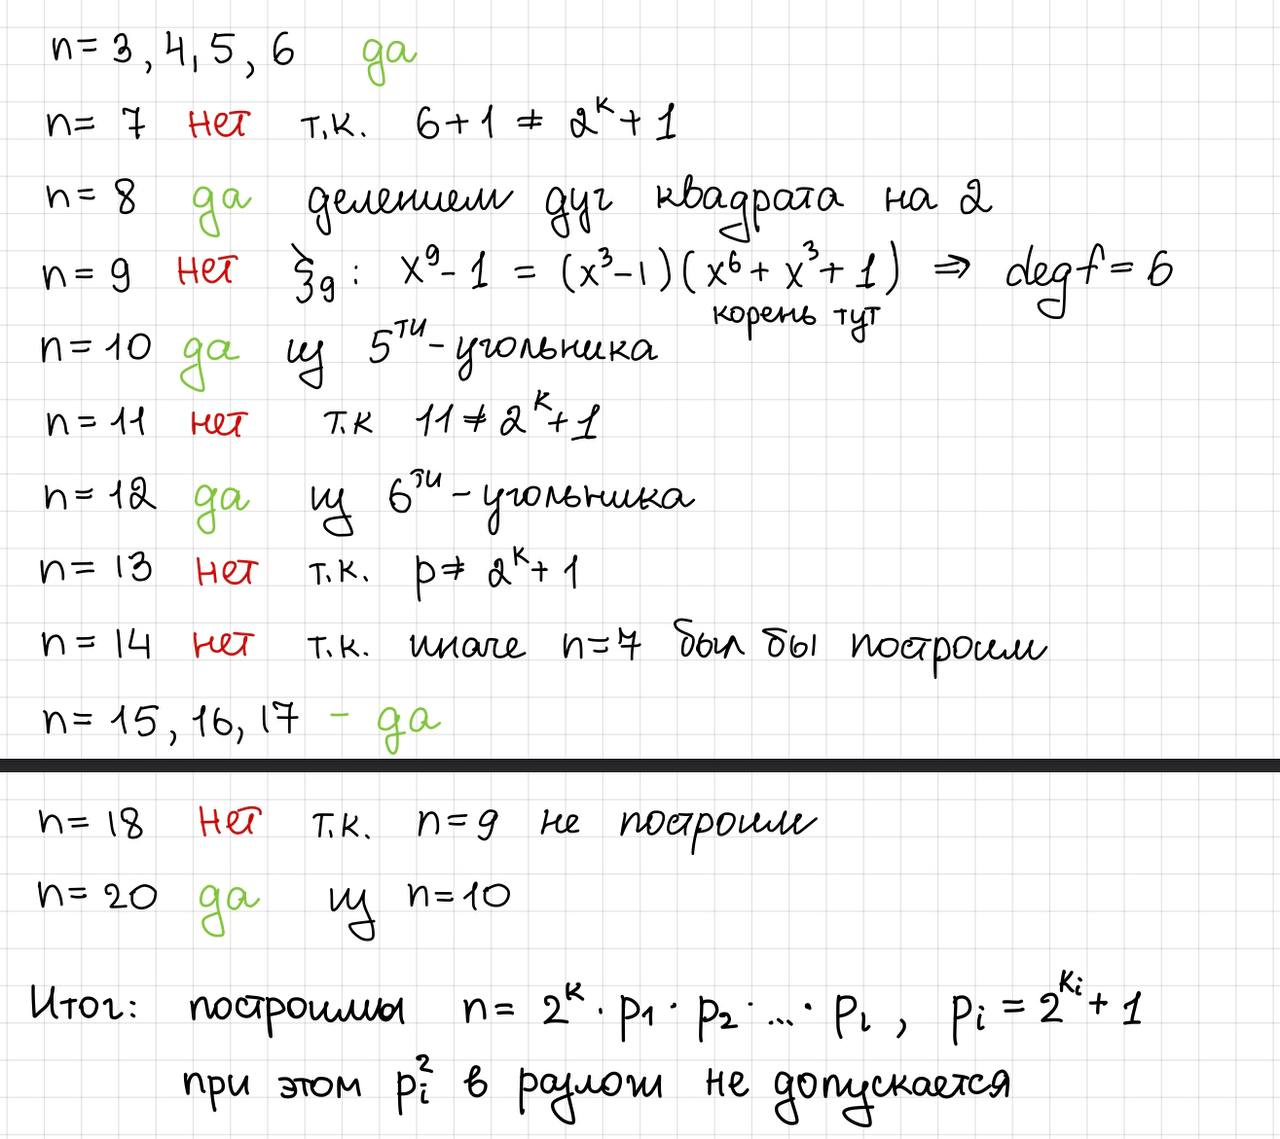
\includegraphics[width=1\linewidth]{sections/Polya/х35.jpg}

\section{Если построены точки $(x_1, \ldots, x_n)$, то можно построить любую точку из поля:}
\begin{itemize}
    \item[а)] $\Q(x_1, \ldots, x_n)$ 
    
    \par \Proof С помощью данных инструментов мы умеем строить следующие действия: если нам даны отрезки $x, y$ то $x+y, x-y, x \cdot y$ (билет 42 на уд). Тогда мы умеем строить $x_1^{k_1}\cdot \ldots \cdot x_n^{k_n}$. Так как мы можем строить сумму, можем построить линейные комбинации таких произведений. Значит осталось научиться строить $x_1 \cdot L, L \in \Q$, но мы умеем строить все рациональные точки (билет 42 на уд), значит мы умеем строить все из $\Q(x_1, \ldots, x_n)$ \EndProof
    
    \item[б)] $K \supset \Q(x_1, \ldots, x_n)$ - квадратичное расширение
    
    \par \Proof Так как $K$ — квадратичное расширение, значит минимальный неприводимый многочлен имеет вид $z^2+az+b=0 \Rightarrow z = \frac{-a \pm \sqrt{a^2-4b}}{2a}$, но все эти действия воспроизводимы (построение корня и частного см. в конце билета), а значит $z$ построим, то есть мы умеем строить любой элемент из квадратичного расширения. \EndProof
\end{itemize}

\par \textbf{Построение корня:} Пользуемся тем, что высота в прямоугольном треугольнике равна среднему геометрическому отрезков гипотенузы - строим отрезок длины $a+1$, на расстоянии 1 от какого-то конца проводим перпендикулярную прямую. Затем берем окружность построенную на нашем отрезке как на диаметре и пересекаем с перпендикуляром. Полученный отрезок высоты будет иметь длину $\sqrt{a}$

\par \textbf{Построение частного:} Воспользуемся подобием треугольников (см. картинку)
\begin{center}
    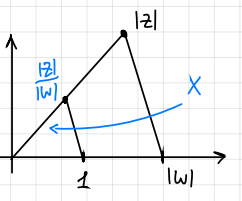
\includegraphics[]{images/4_36_division.png}
\end{center}

$$\frac{w}{1}=\frac{z}{x} \Rightarrow x = \frac{z}{w}$$

\par \Note Помним, что комплексное число можно построить тогда и только когда когда можно построить действительную и мнимую часть (билет 43 на уд), значит частное для них тоже можно построить (домножаем на сопряженное). Корень из комплексных чисел можем извлекать с помощью формулы Муавра (половинный угол мы можем построить)
\newpage{}

\section{Если $\alpha_1, \ldots, \alpha_k$ — алгебраические над F элементы, то}
\begin{itemize}
    \item[а)] $F(\alpha_1, \ldots, \alpha_n) \cong F[\alpha_1, \ldots, \alpha_n]$
    
    \par \Proof Так как $F(\alpha_1, \alpha_2) \cong Quot ((Quot F[\alpha_1])[\alpha_2]) \cong Quot F[\alpha_1, \alpha_2]$, так как $F[\alpha_1, \alpha_2]$ — поле. Аналогично для $n$ элементов. \EndProof
    
    \item[б)] $F[\alpha_1, \ldots, \alpha_n] \supset F$ — конечное расширение степени не больше, чем произведение степеней $m_{\alpha_1}, \ldots, m_{\alpha_n}$
    
    \par \Proof Докажем, что $[F[\alpha_1, \alpha_2]:F]=[F[\alpha_1, \alpha_2]:F[\alpha_1]] \cdot [F[\alpha_1]:F]$. Для этого зададим базисы $F[\alpha_1]:F$ через $1, \alpha_1, \ldots, \alpha_1^{p-1}$, $F[\alpha_1, \alpha_2]:F[\alpha_1]$ через $1, \alpha_2, \ldots, \alpha_2^{q-1}$, где $p,q$ - степени $m_{\alpha_1}, m_{\alpha_2}$ соответственно. Получим, что чтобы разложить элемент из $F[\alpha_1, \alpha_2]$ над базисом $F$, необходимо его разложить изначально по базису $1, \alpha_1, \ldots, \alpha_1^{p-1}$, а затем каждый из этих элементов по базису из $1, \alpha_2, \ldots, \alpha_2^{q-1}$. Получим, что мы разложили элемент по $p \cdot q$ элементному базису, а значит утверждение доказано. Аналогично для $n$ элементного расширения. \EndProof
    
    \item[в)] Любое конечное расширение $K \supset F$ имеет вид $K=F(\alpha_1, \ldots, \alpha_n)$
    
    \par \Proof Рассмотрим произвольный элемент $0 \neq y \in K$. Рассмотрим последовательность $1, y, \ldots, y^n, \ldots$. Так как $[K:F]$ конечно, $\exists n \in \N: \exists \lambda_0, \ldots, \lambda_n: \sum_{i=0}^{n} \lambda_i y^i = 0$. Тогда $y$ — корень многочлена $g(x)=\sum_{i=0}^n \lambda_i x^i = 0$. \EndProof
\end{itemize}
\newpage{}

\section{Полем разложения многочлена $f(x) \in F[x]$ называется минимальное по включению расширение $F$, в котором $f(x)$ раскладывается на линейные множители. Поле разложения существует и имеет степень не больше $n!$.}
\par \Statement Если $f \in F[x]$ — неприводимый многочлен, то в поле $F[x]/(f) \supset F$ у
$f$ есть корень.
\par \Proof Рассмотрим канонический эпиморфизм $\pi: F[x] \rightarrow F[x]/(f)$. Тогда
$f([x])=[f(x)]=[0]$. \EndProof

\par \textbf{Доказательство теоремы:} \Proof Разложим $f$ на неприводимые: $f(x)=f_1(x)\cdot\ldots\cdot f_k(x)$. Рассмотрим $F_1=F[x]/(f_1(x)) \Rightarrow [F_1 : F]=\deg f_1 \leq \deg f$. По доказанному, у $f_1$ есть корень в этом поле. Следовательно $f(x)=(x-\alpha_1) \cdot f_1'(x)\cdot \ldots \cdot f_{k-1}'(x)$. Повторяя процесс получим, что степень искомого расширения $\leq n\cdot(n-1)\cdot\ldots\cdot 2 \cdot 1=n!$ \EndProof

\section{Пусть $K \supset F$ — алгебраическое расширение поля $F$, $\alpha$ алгебраичен над $K$. Тогда $\alpha$ алгебраичен над $F$. а) Если $K \supset L$ и $L \supset F$ — алгебраические расширения, то $K \supset F$ также алгебраическое.}
\par \Statement Пусть $L \supset F$ — алгебраическое расширение поля $F$, $\alpha$ алгебраичен над $L$. Тогда $\alpha$ алгебраичен над $F$
\par \Proof Тогда $\alpha$ является корнем многочлена $f(x) = b_0 + b_1x + \ldots +b_kx^k$, где $b_i \in L$. Рассмотрим расширение $L' = F(b_0, b_1, \ldots, b_k)$. Это конечномерное расширение $F$, которое содержит элементы $b_0, \ldots, b_k$. Элемент $\alpha$ алгебраичен над $L'$, следовательно, $[L'(\alpha) : L']$ конечно. Так как $[L': F]$ конечно, то $[L'(\alpha):F]$ конечно, и следовательно, $L'(\alpha)$ алгебраично над $F$, а значит, и $\alpha$ алгебраичен над $F$. \EndProof
\par \Statement Пусть $K \supset L$ и $L \supset F$ — алгебраические расширения. Тогда $K \supset F$ тоже алгебраическое расширение.
\par \Proof Пусть $\alpha \in K$. Если $\alpha \in L$, то $\alpha$ — алгебраичен над $F$. Пусть $\alpha \in K \setminus L$. Тогда из первого утверждения $\alpha$ алгебраичен над $F$, а значит все эелементы $K$ алгебраичны над $F$, и поэтому расширение $K \supset F$ алгебраическое. \EndProof 


\section{Пусть $\varphi: F \rightarrow L$ — гомоморфизм полей, $\alpha$ — алгебраический над $F$ элемент, $\beta \in L$ — корень
многочлена $\varphi(m_\alpha)$. Тогда существует единственный гомоморфизм $\psi$, продолжающий $\varphi$ на $F[\alpha]$, причём
$\psi(\alpha) = \beta$.}
\par \Proof Так как $\alpha$ алгебраичен над $F$, $m_{\alpha, F}=\sum_{i=0}^n a_i \alpha^i=0$. Тогда $\varphi(m_{\alpha, F})=\sum_{i=0}^n \psi(a_i) \psi(\alpha)^i=\sum_{i=0}^n \varphi(a_i) \cdot \beta^i = 0$. Существование очевидно.
\par Покажем единственность: предположим, что $\varphi$ тоже удовлетворяет требованиям в условии, тогда получим, что $\sum_{i=0}^n \varphi(a_i) \cdot \beta^i = 0 \Rightarrow$ что получили два многочлена минимальной степени, порождающих идеал вида $I=\{f(x) \in F'(\beta)[x] \: | \: f(\beta)=0\}$. Заметим, что этот идеал простой, а значит $(\psi(m_{\alpha, F})) \sim (\varphi(m_{\alpha, F}))$, но это значит, что $\varphi, \psi$ переводят один и тот же многочлен в тот же самый, а значит и все многочлены в те же самые, а значит они совпадают. Противоречие, из которого вытекает
единственность. \EndProof

\section{Назовём число $x \in C$ алгебраическим, если $x$ алгебраично над $Q$. Множество всех алгебраических чисел обозначим через $L$. Докажите, что $L$ является}
\begin{itemize}
    \item[а)] $L$ - поле
    \par \Proof Рассмотрим $a,b\neq 0 \in L$. Тогда $\Q(a, b)$ — алгебраическое расширение $\Rightarrow a+b, a \cdot b, \frac{a}{b} \in L \Rightarrow L$ — поле. \EndProof
    
    \item[б)] $L$ - алгебраически замкнутое поле
    \par \Proof Рассмотрим $f(x) \in L[x], \deg f \geq 1$. Он раскладывается на линейные множители в $\Comp$. Тогда $L(\alpha) \supset L$ — алгебраическое расширение, поэтому $L(\alpha) \supset \Q$ — алгебраическое расширение, значит $\alpha$ алгебраичен над $\Q$, значит $\alpha \in L$. Значит все корни $f(x)$ лежат в $L \Rightarrow L$ алгебраически замкнуто. \EndProof
    
    \item[в)] $L=\overline{\Q}$
    \par \Proof Так как расширение $L \supset \Q$ алгебраическое и $L$ алгебраически замкнуто, по определению $L=\overline{\Q}$ \EndProof
\end{itemize}
\newpage{}

\section{Пусть $F$ — конечное поле или поле рациональных чисел}
\begin{itemize}
    \item[а)] Можно занумеровать все неприводимые многочлены
    \par \Proof Так как $\Q^\N$ счетно, можно занумеровать вообще все многочлены, а значит и неприводимые в том числе. Для конечных полей еще проще. \EndProof
    
    \item[б)] Имеется цепочка вложений $F=F_0 \subset F_1 \subset \ldots \subset F_n \subset \ldots$, где $F_n$ - поле разложения многочлена $f_n$ над $F_{n-1}$
    \par \Proof Построим цепочку $F=F_0 \subset F_1 \subset \ldots \subset F_n \subset \ldots$, где $F_j$ — поле, в котором $f_1, \ldots, f_j$ раскладываются на линейные множители. Очевидно, она будет подходить под требуемую цепочку. \EndProof
    
    \item[в)] Множество $\tilde{F}=\cup_{i=1}^\infty F_i$ - поле
    \par \Proof Рассмотрим два произвольных элемента $a,b \in \tilde{F}$. Тогда $\exists n: a\in F_n, \exists b: b\in F_m \Rightarrow a,b \in F_{max(n,m)}$, так как $F_{max(n,m)}$ — поле, то и $a+b, a\cdot b, \frac{a}{b} \in F_{max(n,m)} \Rightarrow a+b, a\cdot b, \frac{a}{b} \in \tilde{F} \Rightarrow \tilde{F}$ - поле. \EndProof
    
    \item[г)] $\tilde{F}$ алгебраически замкнуто
    \par \Proof Рассмотрим $f(x) \in \tilde{F}[x], \deg f \geq 1$. Он раскладывается на линейные множители в $\Comp$. Тогда $\tilde{F}(\alpha) \supset \tilde{F}$ — алгебраическое расширение, поэтому $\tilde{F}(\alpha) \supset F$ — алгебраическое расширение, значит $\alpha$ алгебраичен над $F$, значит $\alpha \in \tilde{F}$. Значит все корни $f(x)$ лежат в $\tilde{F} \Rightarrow \tilde{F}$ - алгебраически замкнуто. \EndProof
    
    \item[д)] $\overline{F}=\tilde{F}$
    \par \Proof Так как расширение $\tilde{F} \supset F$ алгебраическое и $\tilde{F}$ алгебраически замкнуто, по определению $\tilde{F}=\overline{F}$. \EndProof
\end{itemize}

\newpage{}

\section{Положим $K = Q[\sqrt[3]{2}, \omega]$. Как мы знаем, $K$ — поле разложения многочлена $f(x) = x^3 − 2$.}
\begin{itemize}
    \item[а)] Пусть $g \in Aut(K)$. Какие значения может принимать $g(\sqrt[3]{2})$?
    \par \Proof Так как $(\sqrt[3]{2})^3-2=0 \Rightarrow g^3(\sqrt[3]{2})=2 \Rightarrow g$ переводит $\sqrt[3]{2}$ в корни многочлена $x^3-2$. Тогда $g(\sqrt[3]{2}) \in \{\sqrt[3]{2}, \omega \sqrt[3]{2}, \omega^2 \sqrt[3]{2}\}$. \EndProof
    
    \item[б)] Элемент $Aut(K)$ однозначно задаётся перестановкой корней многочлена $f(x)$
    \par \Proof Корня три $x_1, x_2, x_3$, а значит перестановок 6, а значит если задать перестановку корней $\sigma$, то получим, что $g(x_i)=g(\sigma(x_i))$, а это автоморфизм (проверить вручную нетрудно). Тогда по перестановке можно однозначно задать элемент из $Aut(K)$. \EndProof
    
    \item[в)] Группа $Aut(K)$ изоморфна $S_3$
    \par \Proof Так как данное нам поле — поле разложения многочлена $x^3-2$, расширение нормально. Тогда с учетом того, что степень расширения 6, количество автоморфизмов тоже 6. Тогда группа Галуа и есть $S_3$. \EndProof

    \item[г)] Рассмотрим подгруппу $A_3 \subset S_3$. Найдите поле $K^{A_3}$
    \par \Proof Рассмотрим $g \in Aut(K)$, которая соответствует циклу $(123)$. Тогда $g(\omega)=g(\frac{x_2}{x_1})=\frac{g(x_2)}{g(x_1)}=\frac{x_3}{x_2}=\omega$. Из соображения размерности получим, что $K^{A_3}=\Q(\omega)$. \EndProof
    
    \item[д)] Рассмотрим три подгруппы $H$, каждая из которых порождена одной транспозицией. Найдите $K^H$ для каждой такой подгруппы
    \par \Proof Проделав то же самое для перестановок (132, 213, 321) можно получить, что $\omega$ ни во что хорошее не перейдет (как и любая линейная комбинация), а значит $K^H=\Q$(корень который не участвует в транспозиции). \EndProof
    
    \item[е)] Расширение $K$ имеет четыре нетривиальных подполя, причём эти поля соответствуют подгруппам $S_3$. Более того, нормальным подгруппам $H \subset S_3$ соответствуют нормальные расширения $K^H \supset \Q$.
    \par \Proof Нетривиальные подгруппы из $S_3$ : $(123),(23),(12),(13)$. Тогда для $(23)$ получим, что $\omega \rightarrow \overline{\omega}$. И для нее $K^H=\Q(\sqrt[3]{2})$. Аналогично, рассмотрев подгруппу из $(x_ix_j), K^H=\Q(x_k)$, где $i,j,k$ — различные элементы из $1, 2, 3$. Тогда мы описали для нормальных подгрупп из двух элементов все, а для (123) описано в пункте г). \EndProof 
\end{itemize}
\newpage{}

\section{Конечные поля. Единственность поля из $p^n$ элементов.}
\Th Для любого простого числа $p$ и $n \in \N$ существует конечное поле $F$ такое, что $|F| = p^n$.

\Proof 
	Рассмотрим многочлен $x^{p^n} - x \in \Z_p[x]$ и его поле разложения $L$. Поскольку формальная производная этого многочлена равна $-1$, у него нет кратных корней. Проверим, что $L$ состоит только из корней многочлена $x^{p^n} - x$. Пусть $\alpha, \beta \in L \backslash \{0\}$ "--- нетривиальные корни многочлена. Тогда, по уже доказанному утверждению:
	\begin{itemize}
		\item $(\alpha + \beta)^{p^n} = \alpha^{p^n} + \beta^{p^n} = \alpha + \beta$
		\item $(\alpha\beta)^{p^n} = \alpha^{p^n}\beta^{p^n} = \alpha\beta$
		\item $(-\alpha)^{p^n} = (-1)^{p^n}\alpha^{p^n} = -\alpha^{p^n} = -\alpha$
		\item $(\alpha^{-1})^{p^n} = (\alpha^{p^n})^{-1} = \alpha^{-1}$
	\end{itemize}

	Значит, корни многочлена $x^{p^n} - x$ образуют $L$, поэтому $|L| = p^n$.
\EndProof

\Note Нетрудно проверить, что поле разложения многочлена единственно с точностью до изоморфизма. Но любое конечное поле порядка $p^n$ состоит в точности из корней многочлена $x^{p^n} - x \in \Z_p[x]$. Значит, поле порядка $p^n$ существует и единственно с точностью до изоморфизма.

\section{Группа автоморфизмов конечного поля.}
\Th Пусть $F$ "--- конечное поле, $f \in F[x]$ "--- неприводимый многочлен. Тогда $f$ не имеет кратных корней над $\overline{F}$.

\Proof 
Пусть это не так, тогда $(f, f') \not\sim 1$. Тогда, в силу неприводимости многочлена $f$, $f' = 0$. Значит, $f$ имеет вид $f = a_mx^{mp} + \dotsc + a_1x^p + a_0$ для некоторых $a_0, \dotsc, a_m \in F$. Но тогда $f = (a_mx^{m} + \dotsc + a_1x + a_0)^p$, что противоречит его неприводимости.
\EndProof

\Th $\Aut\F_{p^n} \cong \Z_n$.

\Proof
Обозначим через $\phi \in \Aut\F_{p^n}$ \textit{автоморфизм Фробениуса}, имеющий вид $\phi(x) := x^p$ для всех $x \in \F_{p^n}$. Очевидно, $\phi$ сохраняет операции, инъективность же выполнена потому, что $\ke\phi = \{0\}$, и ее достаточно для биективности, поскольку $\F_{p^n}$ конечно. Заметим также, что $\F_{p^n}^\phi = \{a \in \F_{p^n} : a^p = a\} = \Z_p$.
	
	С одной стороны, $\phi^n = \id$. С другой стороны, $\forall k \in \{1, 
	\dotsc, n - 1\}:$ равенство $\phi^k(x) = x$ выполнено только для таких элементов поля $\F_{p^n}$, которые являются корнями многочлена $x^{p^k} - x \in \Z_p[x]$.  Но $|\Aut\F_{p^n}| = |\Aut_{\Z_p}\F_{p^n}| = [\F_{p^n} : \Z_p] = n$ в силу нормальности расширения $\F_{p^n} \supset \Z_p$, поэтому $\Aut\F_{p^n} = \gl\phi\gr = \{\id, \phi, \dotsc, \phi^{n-1}\} \cong \Z_n$.

\EndProof 

\section{Описание промежуточных подполей конечного поля при помощи группы автоморфизмов.}
\begin{corollary}
	Подполя в $\F_{p^n}$ имеют вид $\F_{p^k}$, где $k \mid n$, причем для каждого $k \mid n$ подполе порядка $p^k$ существует и единственно.
\end{corollary}

\begin{proof}
	Подполя в $\F_{p^n}$ биективно соответствуют подгруппам в $\Aut\F_{p^n} \cong \Z_n$. Но все подгруппы в $\Z_n$ имеют вид $k\Z_n$ для $k \mid n$, причем подгруппа каждого порядка единственна. Легко проверить, что тогда подгруппа в $\Aut\F_{p^n}$ индекса $k$ соответствует в точности подполю $\F_{p^k} \subset \F_{p^n}$ при каждом $k \mid n$, причем единственному, и других подполей в $\F_{p^n}$ нет.
\end{proof}
\newpage{}

\section{Верно ли, что неприводимый многочлен над $\F_p$ делит многочлен $x^{p^n} - x$ тогда и только тогда, когда его степень делит n?}
\input{sections/Kolya/4_47}

\section{Количество неприводимых многочленов степени n над $F_p$}
\Th
	Обозначим через $d_n$ число многочленов степени $n$, неприводимых над $\Z_p[x]$. Тогда для любого $n \in \N$ выполено следующее равенство:
	$d_n = \frac{1}{n}\sum\limits_{k \mid n}p^k\mu\left(\frac {n}{k}\right)$

\Proof
	Поле $\mathbb{F}_{p^n}$ является полем разложения многочлена $x^{p^n} - x \in \Z_p[x]$. Рассмотрим разложение $x^{p^n} - x = f_1\dotsb f_s$ на неприводимые сомножители и докажем, что $f_1, \dotsc, f_s \in \Z_p[x]$ -- это в точности все различные неприводимые над $\Z_p[x]$ многочлены степеней $k$ таких, что $k \mid n$.
	
	Многочлены $f_1, \dotsc, f_s$ различны потому, что у $x^{p^n} - x$ нет кратных корней. Рассмотрим теперь многочлен $f_i$ степени $k_i$ для произвольного $i \in \{1, \dotsc, s\}$ и его произвольный корень $\alpha \in \mathbb{F}_{p^n}$. Тогда расширение $\Z_p(\alpha)$ имеет степень $k_i$. Но $\Z_p(\alpha) \subset \mathbb{F}_{p^n}$, поэтому $k_i \mid n$. С другой стороны, если $f \in \Z_p[x]$ -- неприводимый многочлен степени $k \mid n$ и $\alpha \in \overline{\Z_p}$ -- его корень, то $|\Z_p(\alpha)| = p^k$, поэтому $\alpha \in \mathbb{F}_{p^k} \subset \mathbb{F}_{p^n}$. Значит, $f = f_i$ для некоторого $i \in \{1, \dotsc, s\}$.
	
	Подсчитывая число корней в левой и правой части равенства $x^{p^n} - x = f_1\dotsb f_s$, получаем, что $p^n = \sum\limits_{k \mid n}k d_k$. Тогда, по формуле обращения Мебиуса, $n d_n = \sum_{k \mid n}p^k\mu(\frac{n}{k})$, что и требовалось.
\EndProof

\newpage{}